\section{Model}

\subsection{Statement of the model} We developed a model which consists of 2 dynamic variables representing the line density of lamin A/C, $a(t)$, and lamin B, $b(t)$, as functions of time, $t$ on a simple closed curve in 2D, $s(t)$, enclosing an area, $\mathcal{A}(t)$. The details of laminA/C (B)  assembly and dissassembly into the lamina are unknown, we assume usual assembly kinetics and allow for possible feedback in the dissassembly terms. It is known that lamin proteins are not confined to the nuclear lamina, but exist in the nucleoplasm where they may be performing other functions, including gene regulation. [REFERENCE] We will assume there is a pool of nuclear lamins which exchanges dynamically with the the lamins in the nuclear lamina. The resulting equations are:

\begin{align}
\dfrac{\partial a}{\partial t} = \dfrac{k_{on}^a}{\mathcal{A}(t)} a_{nuc} - k_{off}^a (s,b)a\\[7pt]
\dfrac{\partial b}{\partial t} = \dfrac{k_{on}^b}{\mathcal{A}(t)}b_{nuc} - k_{off}^b  (s,a)b \label{eq::laminaKinetics}
\end{align}

The parameters $k_{on}^a , k_{on}^b$  govern assembly of lamin A/C, and lamin B into the lamina, respectfully. The functions $k_{off}^a (s,b) = k_{off}^{0a} + \Phi_a(s,b)$ and $ k_{off}^b(s,a)  = k_{off}^{0b} + \Phi_b(s,a)$ describe laminar turnover with possible feedback terms arising from $\Phi$. The nuclear pools of lamin A/C (B) are labelled by $a_{nuc} (b_{nuc})$. We therefore have the following conservation of lamin equations. 

\begin{align}
a_{tot}= \int_0^{\mathcal{L}_0} a(s,t) ds + a_{nuc}\\
b_{tot} = \int_0^{\mathcal{L}_0} b(s,t) ds + b_{nuc}
\end{align}

These equations are coupled to a mechanical description of the lamina via the energy functional:

\begin{align}
\mathcal{E} = \mathcal{E}_{stretch} + \mathcal{E}_{pressure} +\mathcal{E}_{bending} + \mathcal{E}_{cytoskeleton} + k_B\mathcal{T} \xi
\end{align}
Where 
\begin{align}
\mathcal{E}_{stretch} = \displaystyle \int_0^{\mathcal{L}_0} \dfrac{1}{2} (\mathcal{G}_a(a(s)) +\mathcal{G}_b(b(s)) )\left( \left |\left| \dfrac{\partial \vec{x} }{\partial s} \right|\right| - 1\right)^2 ds \\
\mathcal{E}_{pressure}  = \mathcal{P} \left( \dfrac{\mathcal{A}}{\mathcal{A}_0} -1\right)^2  \\
\mathcal{E}_{bending} = \displaystyle\int_0^{\mathcal{L}_0} \dfrac{1}{2 } (\mathcal{M}_a(a(s)) + \mathcal{M}_b (b(s)) \left|\left| \dfrac{\partial^2 \vec{x}}{\partial s^2} \right|\right|^2 ds\\
\mathcal{E}_{cytoskeleton} = \displaystyle\int_0^{\mathcal{L}_0} \mathcal{F}_{cyto} (a(s))\Theta (\theta) || \vec{x} || ds 
\end{align}
and \[ \Theta (\theta) = \dfrac{e^{\cos(2\theta)/\sigma_{\rm VM }}}{\int_0^{ 2\pi} e^{\cos(2\theta)/\sigma_{\rm VM}}d \theta} \]

The lamina is modeled as an elastic material where the first term, $\mathcal{E}_{stretch}$ corresponds to laminar surface tension. The next term, $\mathcal{E}_{pressure}$ is hydrostatic pressure from the nucleus possibly due to chromatin [REFERENCE]. The third term,$\mathcal{E}_{bending}$  is bending resistance terms due to lamin-lamin crosslinking. It is know that there are non-negligible forces produced by the cellular cytoskeleton(actin and microtubules) which act on the lamin via nuclear transmembrane proteins [REFERENCES] and so the fourth term, $\mathcal{E}_{cytoskeleton}$, is due to this. Finally we include a term for thermal fluctuations generalized to 2D, $k_B\mathcal{T} \xi$. 


A complete list of parameter descriptions can be found in Table ~\ref{tab:nucmodelparameters}

\begin{table}[t!]
\caption{Mechanical parameters.}\centering \label{tab:nucmodelparameters} 
\begin{tabular}{ c  l  l}
\hline
Symbol & Dimensions & Meaning \\
\hline
$\mathcal{G}_a $ & [pN]  & Stretch modulus associated with lamin A/C \\
$\mathcal{G}_b$& [pN] & Stretch modulus associated with lamin B\\
$\mathcal{P}$ & [pN$\mu$m] & Bulk modulus \\
$\mathcal{A}_0$  & [$\mu$m$^2$ & Resting area of nucleus\\
$\mathcal{M}_a$ & [pN$\mu$m$^2$] &  Bending modulus associated with lamin A/C\\
$\mathcal{M}_b $ & [pN$\mu$m$^2$] &  Bending modulus associated with lamin B\\
$\theta$ &  [rad] & Angle \\
$\mathcal{F}_{cyto}$ & [pN /$\mu$m] & Force line density of the cytoskeleton (if negative --pull/ if positive --push)\\
$\sigma_{\rm VM}$ & [dimensionless] & Concentration of distribution of cytoskeletal force\\
\hline
\end{tabular}
\end{table}


We non dimensionalized the system by choosing characteristic scales for length, time, energy and amount of lamin. The details of this non-dimensionalization procedure can be found in Appendix ~\ref{sec:project2}. The resulting non-dimensional system is expressed by the following system of equations:

\begin{align}
\dfrac{\partial A}{\partial \tau} &= \kappa_{on}\dfrac{1}{\lambda (\tau)} A_{nuc}  - (\kappa_{off}+ \phi_A (S,B)) A,  \\[10pt]
\dfrac{\partial B}{\partial \tau} &= \dfrac{1}{\lambda (\tau)} B_{nuc}  - (1+ \phi_B (S,A)) B  \\[10pt]
\end{align}

With Energy 
\begin{align}
 E = \displaystyle \int_0^{2 \sqrt{\pi}} \dfrac{1}{2} (G_A(A(S))+ G_B(B(S)))\left( \left |\left|  \dfrac{\partial \vec{\chi} }{\partial S} \right|\right| - 1\right)^2  dS + \Pi \left(\dfrac{\lambda(\tau)}{\lambda_0} -1\right)^2\\[10pt]
 +\displaystyle\int_0^{2\sqrt{\pi}} \dfrac{1}{2 } (M_A(A(S))+ M_B(B(S)))\left|\left| \dfrac{\partial^2 \vec{\chi}}{\partial S^2} \right|\right|^2 dS\\[10pt]
+ \displaystyle\int_0^{2\sqrt{\pi}} F_{cyto}(A(S))\Theta (\theta) \left|\left| \vec{\chi} \right|\right| dS +k_BT \xi
\end{align}

A description of non dimensional variables can be found in Table ~\ref{tab:nondimvar} and parameters in Table ~\ref{tab:nondimpar}.

\begin{table}[t!]
\caption{Non-dimensionalized variable.}\centering \label{tab:nondimvar} 
\begin{tabular}{ l  l}
\hline
Symbol  & Meaning \\
\hline
$A$ & Laminar non-dimensionalized density of Lamin A/C \\
$B$ & Laminar non-dimensionalized density of Lamin B  \\
$A_{nuc}$ & Nucleoplasmic lamin A/C \\
$B_{nuc}$ & Nucleoplasmic lamin B\\
$S$ & Non-dimesionalized position of the lamina\\
$\lambda(\tau)$ & Non-dimesionalized area of nucleus\\
\hline
\end{tabular}
\end{table}


\begin{table}[t!]
\caption{Non-dimensionalized parameters.}\centering \label{tab:nondimpar} 
\begin{tabular}{ l  l}
\hline
Symbol  & Meaning \\
\hline
$\kappa_{on}$ &  Non-dimesionalized rate constant associated with lamin A/C incorporation into the lamina\\
$\kappa_{off}$ &  Non-dimesionalized rate constant associated with lamin A/C dissociation from the lamina\\
$G_A$ & Non-dimensionalized stretch modulus associated with lamin A/C \\
$G_B$ &  Non-dimensionalized stretch modulus associated with lamin B\\
$\Pi$ &  Non-dimensionalized bulk modulus \\
$\lambda_0$ & Resting non-dimensionalized area of nucleus\\
$M_A$ & Non-dimensionalized bending modulus associated with lamin A/C\\
$M_B$  & Non-dimensionalized bending modulus associated with lamin B\\
$\theta$ & Angle   \\
$F_{cyto}$ &  Non-dimensionalized force line density of the cytoskeleton (if negative --pull/ if positive --push) \\
\hline
\end{tabular}
\end{table}


\subsection{Numerical implementation of the model}

The model is implemented in Matlab by discretizing the 2D simple closed curve into a series of nodes connected by linear springs with an elastic modulus dependent on the amount of lamins at the two nodes on either side of each spring. We solve the ODE systems using the forward Euler method. The energy minimization is done using a Markov chain Monte Carlo method at each step forward in time. 

\subsection{Tuning the model}

Many of the mechanical parameters of the model are unknown because they are difficult or impossible to measure experimentally. We therefore have to tune the parameters in our model using some data. We used data from a series of experiments conducted on rat cardiomyocytes grown on fibronectin islands of various shapes and sizes as shown in Fig. \ref{fig::nancycells} [REFERENCE NANCY DREW PAPER]. The features we extracted from the images are cellular aspect ratio, F-actin OOP (a measure of the anisotropy in the F-actin network), nuclear eccentricity, nuclear area, nuclear perimeter. 

\begin{figure}[h]
\centering
\captionsetup{width=.9\linewidth}
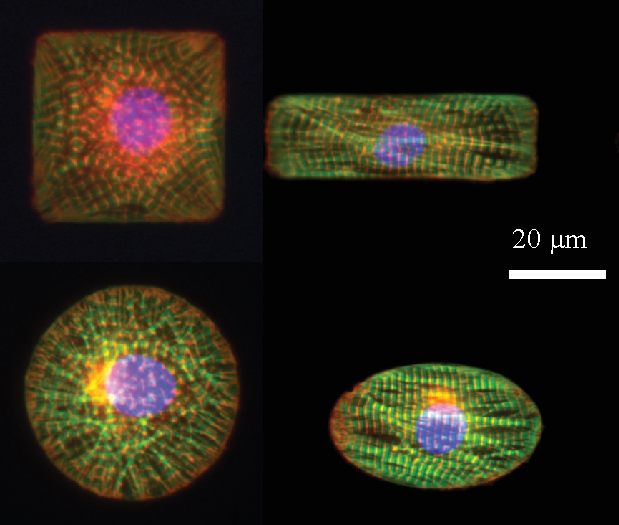
\includegraphics[width=4.5in]{Project3/figs/nancycells.pdf}
\caption{Nancys cells.}
\label{fig::nancycells}
\end{figure}

In order to extract information about the correlations between these features we plotted each against the others in a scatter plot matrix, see Fig. ~\ref{fig::scattermatrix}. From here we chose three patterns in the data to fit our model. We first chose a subset of the cell which have low F-actin OOP and tuned parameters to match the histograms of nuclear area and nuclear perimeter in both mean and standard deviation. This subset of cells was chosen so that we could assume isotropic cytoskeletal force and therefore set it to 0. Once these parameters were tuned (Fig. ~\ref{fig::histos}), we returned to the entire data set and tuned our model to match the eccentricity vs F-actin OOP plot, see Fig. ~\ref{fig::eccopp}. As this gave us an order of magnitude estimation of $F_{cyto}$ which is in fact a ratio of two dimensional quantities, we were able to obtain order of magnitude estimates for all our mechanical parameters. These estimates are summarized in Table ~\ref{}.

\begin{figure}[h]
\centering
\captionsetup{width=.9\linewidth}
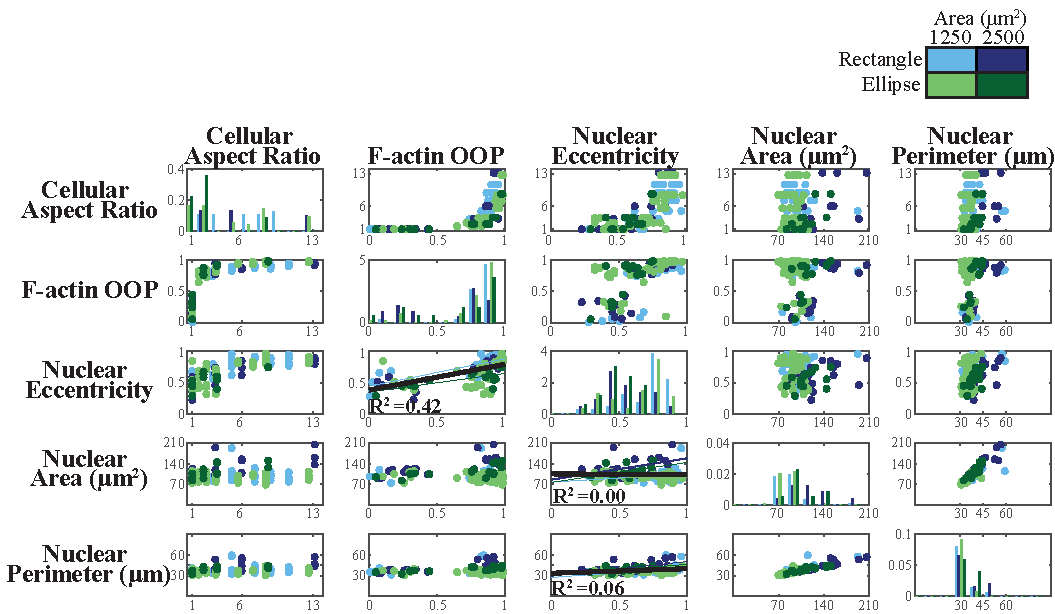
\includegraphics[width=6in]{Project3/figs/Nancy_data.pdf}
\caption{scattermatrix}
\label{fig::scattermatrix}
\end{figure}


\begin{figure}[h]
\centering
\captionsetup{width=.9\linewidth}
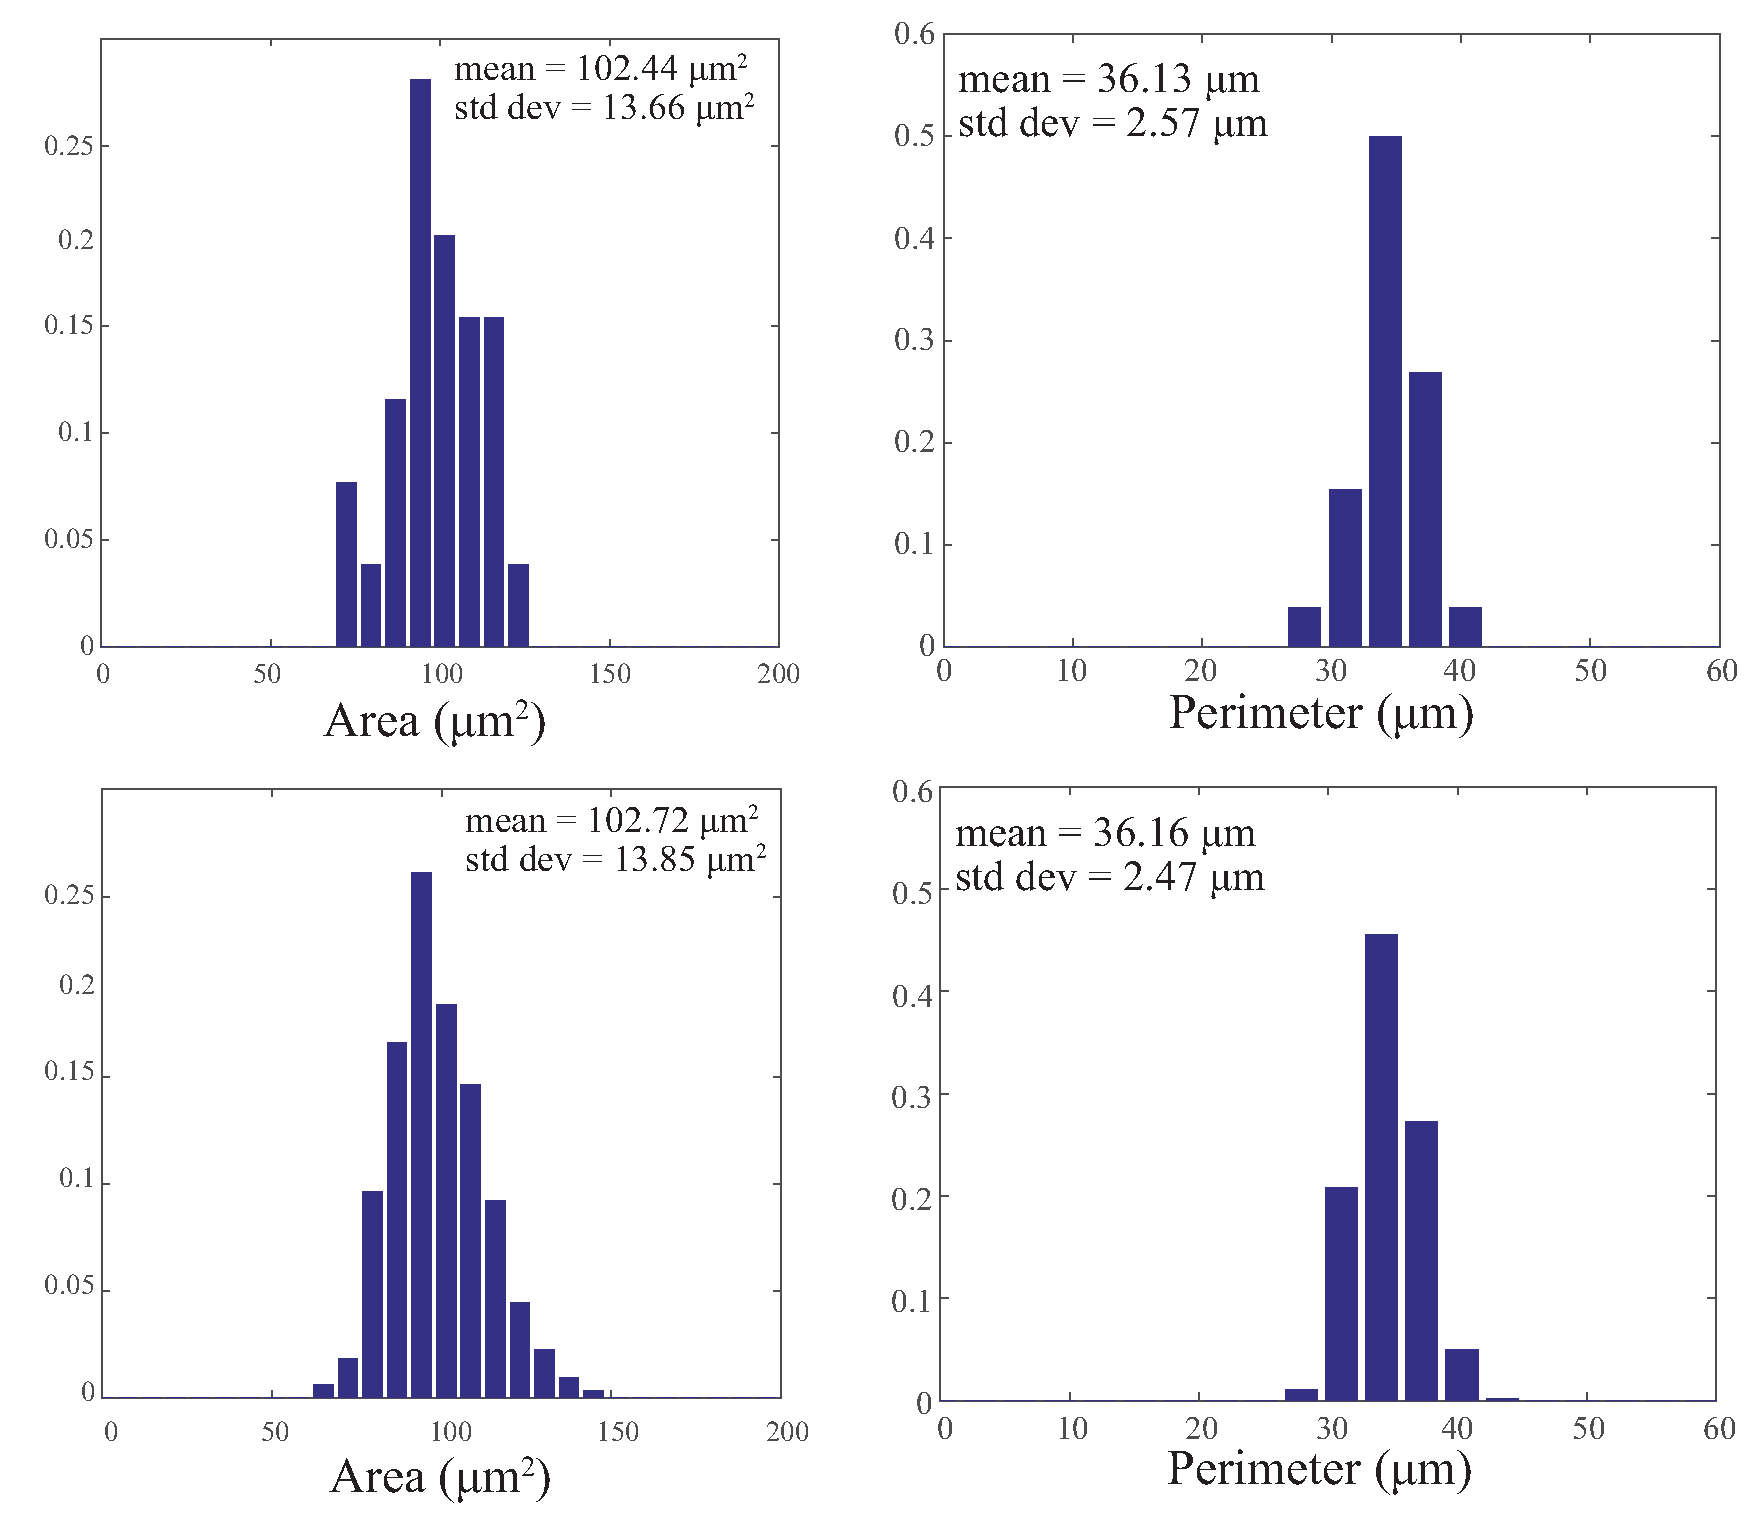
\includegraphics[width=4.5in]{Project3/figs/matching_histograms_areaandperim.eps}
\caption{matched histograms}
\label{fig::histos}
\end{figure}

\begin{figure}[h]
\centering
\captionsetup{width=.9\linewidth}
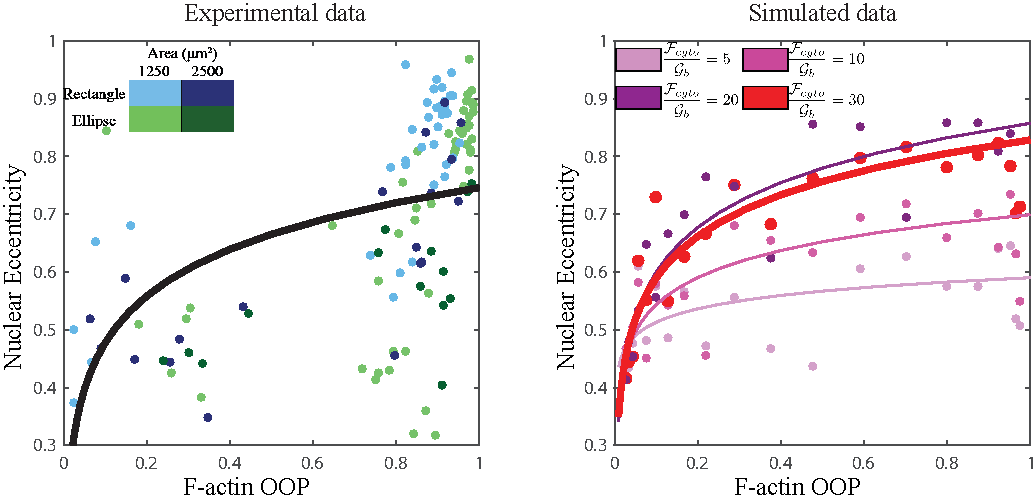
\includegraphics[width=4.5in]{Project3/figs/EccentricityvsOOP.pdf}
\caption{finding F cyto}
\label{fig::eccopp}
\end{figure}



